
\begin{frame}{A small example}
\begin{center}

\includegraphics[width=.15\textwidth]{img/boy1.png} \qquad \qquad

\includegraphics[width=.15\textwidth]{img/boy2.png}

\vspace*{3ex}


\includegraphics[width=.15\textwidth]{img/computer.png} \qquad \qquad

\includegraphics[width=.15\textwidth]{img/mother.png}
\end{center}

\begin{itemize}
\item Two brothers, Alfred and Ben; both need to 
\begin{itemize}
\item[-] Read about an algorithm before
\item[-] programming it on a computer
\end{itemize}
\item Their mother needs to do work on a computer as well
\item Only one computer is available
\end{itemize}
\end{frame}

\begin{frame}[fragile]{Model}

\begin{lstlisting}
int: T = 5; set of int: TASK = 1..T;
set of int: HORIZON = 0..50;
array[TASK] of var HORIZON: s; % start times
array[TASK] of var HORIZON: e; % end times 
var HORIZON: makeSpan; 
int: readAlfred = 1; int: codeAlfred = 2;
int: readBen = 3; int: codeBen = 4; int: workMother = 5;

% durations
array[TASK] of int: d = [5, 2, 3, 8, 12];

constraint forall(t in TASK) (s[t] + d[t] = e[t]);
constraint forall(t in TASK) (e[t] <= makeSpan);
constraint e[readAlfred] <= s[codeAlfred] /\ e[readBen] <= s[codeBen];

set of TASK: conflicting = {codeAlfred, codeBen, workMother};
constraint disjunctive( [s[t] | t in conflicting], 
                         [d[t] | t in conflicting] ); 
solve minimize makeSpan;
\end{lstlisting}
\end{frame}

\begin{frame}[fragile]{Solution}

\begin{lstlisting}
int: readAlfred = 1; int: codeAlfred = 2;
int: readBen = 3; int: codeBen = 4; int: workMother = 5;
set of TASK: conflicting = {codeAlfred, codeBen, workMother};
array[TASK] of int: d = [5, 2, 3, 8, 12];
\end{lstlisting}
\small 
\begin{verbatim}
s = array1d(1..5 ,[0, 20, 0, 12, 0]);
e = array1d(1..5 ,[5, 22, 3, 20, 12]);
makeSpan = 22;
\end{verbatim}

\tikzset{
    task/.style={rounded corners, text centered, minimum height=3.8ex,rectangle,anchor=south west},
    task1/.style={task,draw=black, top color=isseorange!5, bottom color=isseorange!30},    
    task2/.style={task,draw=black, top color=ForestGreen!5, bottom color=ForestGreen!30},
    task3/.style={task,draw=black, top color=BrickRed!5, bottom color=BrickRed!30},
}
 \hspace*{-2ex}
 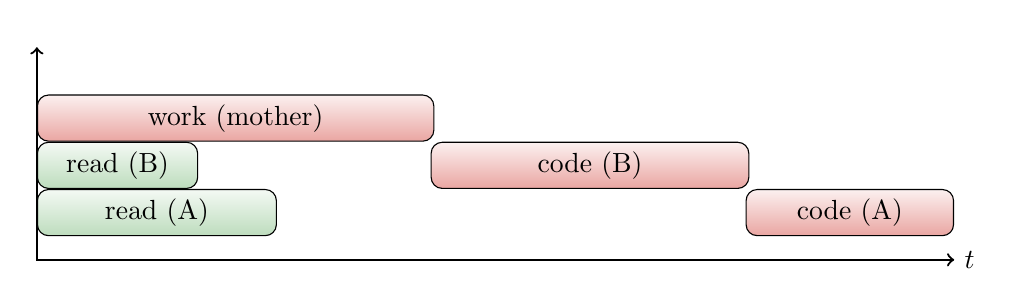
\begin{tikzpicture}[x=1cm,y=1cm]
    % Draw axes
    \draw [<->,thick] (0,2.7) node (yaxis) [above] {}
        |- (11.65,0) node (xaxis) [right] {$t$};    

  %  \node[task1] at (1,0.5) { cut onions };        
    \node[task2,text width=2.8cm] at (0,0.3) {read (A)};         
    \node[task2,text width=1.8cm] at (0,0.9) {read (B)};         

    \node[task3,text width=4.8cm] at (0,1.5) {work (mother)};         
	\node[task3,text width=2.4cm] at (9,0.3) {code (A)};         
    \node[task3,text width=3.8cm] at (5,0.9) {code (B)};        
   
  %  \node[task3] at (2,1.5) { cook spaghetti };  

\end{tikzpicture}
 
\end{frame}

